\documentclass[11pt]{article}
\usepackage[utf8]{inputenc}

\usepackage{geometry}
\geometry{a4paper}

\usepackage{graphicx}
\usepackage{hyperref}
\usepackage[parfill]{parskip}
\usepackage{amsmath, amssymb}
\usepackage{fdsymbol}
\usepackage{color,soul}

% remove section numbering
\makeatletter
\renewcommand{\@seccntformat}[1]{}
\makeatother

% make subsubsection italic
\usepackage{sectsty}
\subsubsectionfont{\itshape}

\renewcommand{\arraystretch}{1.4}

\title{Probability Theory \& Statistics}
\date{}
\author{}

\begin{document}
\maketitle
\clearpage

\section{None-Naïve Probability}

\subsection{Prerequisites}

\begin{itemize}
\item Events
\item Counting
\end{itemize}

\subsection{Definition}

General definition of probability: 
A \emph{probability space} consists of a \emph{sample space} \(S\) 
and a \emph{probability function} \(P\) 
that takes an event \(A \subseteq S\) as an input and returns \(P(A)\), 
a real number between 0 and 1, as its output.%
\footnote{Numbers are the fourth fundamental object in probability theory.} 

The function \(P\) must satisfy the two axioms:
\begin{align}
P(\varnothing) = 0,\ P(S) = 1
\end{align}
and
\begin{align}
P\left( \bigcup_{j = 1}^{\infty}A_{j} \right) = \sum_{j = 1}^{\infty}{P(A_{j})}
\end{align}
where \(A_{j}\) are disjoint events.
The symbol \(\varnothing\) denotes the empty set \(\varnothing=\{\cdot\}\). 
The symbol \(\cup\) denotes the \emph{union} of events, 
the combination of outcomes from sets.

\begin{figure}[h!]
\centering
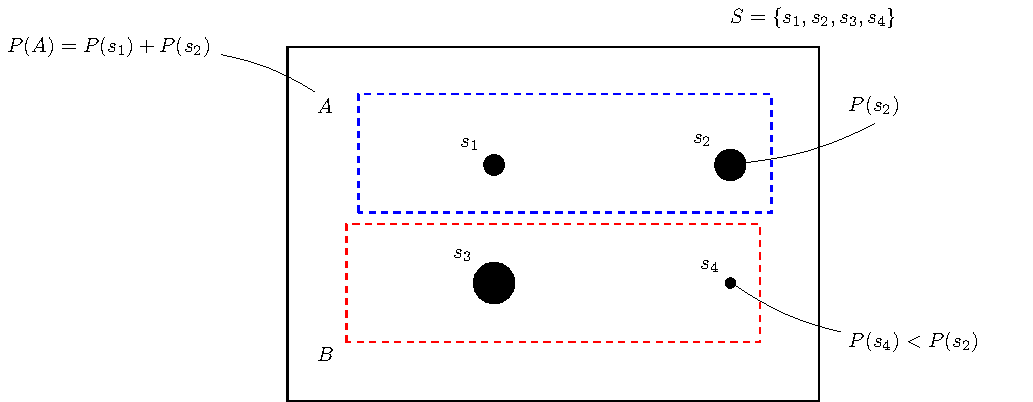
\includegraphics[width=0.9\linewidth]{tikz/figure1}
\caption{%
Outcomes with different likelihoods of occurring.
The event \(A\) is the set \(\{s_1, s_2\}\) with probabilities \(p_1=P(s_1)\) and
\(p_2=P(s_2)\),
for \(p_1 \neq p_2\).
}
\label{fig:outcomes}
\end{figure}

\subsection{Interpretation}

\subsubsection{Axioms}

The none-naïve definition says that probability 
behaves like the mass of marbles. 
The mass of an empty pile of marbles is 0,
and the total mass of all marbles is 1. 
Moreover, 
if we add none-overlapping piles of marbles, 
we get their total mass by combining the individual masses. 

Unlike in the naïve definition, 
we can now have marbles with different masses, 
and have a countably infinite number of outcomes provided their mass sums to 1.
The larger the mass, 
the more likely the event will occur (the more likely the 
marble will be picked from the imaginary bag). 

An alternative interpretation considers the outcomes 
as distinguishable regions on a map. 
If we place our finger at random anywhere on the map, 
the larger the region, 
the more likely we choose that country.
Let \(A\) be the event we place our finger on 
North America with \(P(A)=0.163\),
and let \(B\) be the event we place our finger on 
the UK with \(P(B) = 0.00167\).
Since (we assume) we cannot place our 
finger on both North America and the UK, 
the events are \emph{disjoint}.
The probability we randomly place our finger on \emph{either} 
North America \emph{or} the UK is given by
\begin{align}
P(A \cup B) = P(A) + P(B) = 0.16467,
\end{align}
since their combined regions linearly sum,
consistent with the non-naïve definition.%
\footnote{%
The event \(A\) is the set of outcomes \(A = \{s_1, s_2, \ldots\}\), 
where \(s_1\) is Canada, 
\(s_2\) is the US etc..
}

In both analogies, 
the ``randomness'' comes from performing the experiment, 
by randomly placing a finger on the globe, 
and \emph{randomly sampling} outcomes where it is more or less likely to choose a given outcome -- unlike in the naïve definition.

\begin{figure}[h!]
\centering
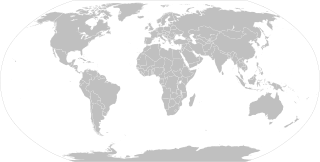
\includegraphics[width=0.75\linewidth]{images/figure2}
\caption{%
Landmass interpretation of the probability function \(P\) assigning a (land)mass to an event.
An experiment corresponds to randomly placing a finger on the map where any given position 
on the map is \emph{equally likely} to be chosen. 
The probability of any given outcome, 
a distinguishable region on the map,
is proportional to the size of the region (analogous to the mass of the marble). 
Events, 
collections of outcomes, 
correspond to continents or collections of regions like the UK.
}
\label{fig:landmass}
\end{figure}

\subsubsection{Probability}

Any function \(P\) mapping events to numbers in the interval \([0,1]\) that satisfies the two axioms 
is considered a valid probability function. 
However, 
the axioms don't tell us how the probability should be interpreted.

The \emph{frequentist} interpretation says that the probability
represents the long-run frequency over a very large number of experiments, 
e.g., if we say a coin has probability ½ of Heads, 
flipping a coin repeatedly for a very long time, 
50\% of the time the coin would land on Heads.%

The \emph{Bayesian} view says that \(P\) represents a degree of belief about an event. 
We can assign a probability to the 
hypothesis ``president X will win the election'' even if it's not 
possible to repeat the same election over and over again.

\section{Discussions}

\subsection{Repeatability}

\emph{What does repeating an experiment mean?}

Repeating an experiment does not necessarily mean 
that the \emph{exact same experiment} is performed over and over
again. 
For example, 
a football game may be regarded as a random experiment in 
the sense that the outcome of the game is uncertain \emph{a priori}; 
however, 
the experiment (the game) is not repeatable as
we surely could not guarantee that each game would be played
under the exact same conditions. 
Nonetheless, 
it is often plausible that a given random experiment 
is \emph{conceptually repeatable}; 
for example,
we might be willing to assume that team A would win 40\% of
its games against team B under a certain set of conditions. 
This ``conceptual repeatability'' is important as it allows us to interpret
probabilities in terms of long-run frequencies.

\subsection{Sampling}

\emph{How is the frequentist interpretation related to the law of large numbers?}

The frequentist interpretation of probability is very loosely related to the law of large numbers.
The law of large numbers (LLN)
and the central limit theorem (CLT) describe the behaviour of sums of random variables, e.g.,
\begin{align}
n\widehat{X} = X_{1} + X_{2} + \cdots
\end{align}
where \(\widehat{X}\) is itself a random variable; 
``hats'' often denote \emph{estimators} where here the average estimates the expectation. 
Note, we haven't yet formally introduced random variables or 
expectations of distributions so we're getting ahead of ourselves!

The \emph{weak law of large numbers} says that...

\begin{quote}
...the sum of a large number of IID
(independently and identically distributed) random variables
converges to the expectation of the distribution
of the random variables.%
\footnote{
There are many interesting things to deduce in this statement: 
in what sense does a sum of random variables (a random variable) converge
towards the expectation (a number)?
We later prove the LLN and attempt to answer this question. 
}
\end{quote}

The CLT tells us that, 
provided the expectation and variance exist and are finite, 
the distribution of the estimator will be Normal! 
This is an astonishing result and well worth thinking about why.

%Try running the following command in R to see this
%
%\begin{align}\text{hist(replicate(1000, sum(runif(1000))))}\end{align}

An important ``real world'' consequence of the LLN and CLT is that they 
theoretically guarantee (under certain conditions) that the average value in the replication 
of some quantity approximates its theoretical average. 
(Note, this wasn't obvious at all until recently).\footnote{Recently in mathematics means in the last 100 years, 
compared to Pythagoras' Theorem that's been known for several millennia.}

That is, if I throw a succession from a fair coin and:
\begin{itemize}
\item the coin has no memory -- so all of the throws are independent
\item and every throw stays fair -- the distribution from which every throw is 
drawn stays the same
\end{itemize}

Then,
\begin{itemize}
\item by LLN, the average number of Heads in the experiment converges to ½. 
\item by CLT, the distribution of the average will be Normal.
\end{itemize}

Thus, generating data from a large number of independent replications of an experiment, 
performed either by computer simulation or in the real world yields estimable results.

What does this have to do with the frequentist interpretation? 
Well, not much really. 
The frequentist interpretation simply tells us how to interpret the function \(P\). 
We don't need to posit anything at all about \(P\) besides that it's a function. 
We don't care if our experiments are independent, 
or from what distribution they come from.
In fact, 
it's almost never true that measurements are IID. 
Nonetheless, we still go out and measure them, and interpret the data as probabilities (either naively or by other means)!

\subsection{Simulation}

\emph{Why should we care about any of this?}

The frequentist interpretation says that if we repeat an experiment a large number of times we can
approximate the probability through counting the favourable outcomes and dividing by the total number of outcomes, i.e.,
by computing the \emph{frequency}.
If we can simulate the experiment in a computer, 
we can study the problem by running the simulated experiment many times.

A beautiful aspect of probability is that it is often possible to study problems via simulation. 
Rather than endlessly debating an answer, 
you can run a simulation and ``see'' the answer. 

In the supporting material, 
we show how to sample from equally and not equally likely outcomes. 
Multiple approaches to solving the Birthday Problem are also provided. 
The calculations and simulations are done in R, 
a free statistical computing environment.

\section{Practice}\label{practice}

1) Events \(A\) and \(B\) are \emph{independent} if
\begin{align}
P(A \cap B) = P(A)P(B)
\end{align}
Give an example of independent events illustrated as marbles in a finite
sample space.

2) Consider the experiment of picking a random point in the unit square
\begin{align}
R = \{(x,y)\ :\ 0 < x < 1,\ 0 < y < 1\}
\end{align}
where the probability of the point being in any particular region
contained within \(R\) is the area of that region, e.g., \(P(A) = ab\),
for a rectangle with sides of length \(a\) and \(b\). Let \(A_{1}\) and
\(B_{1}\) be rectangles contained within \(R\), with areas not equal to
0 or 1. Let \(A\) be the event that the random point is in \(A_{1}\),
and \(B\) be the event that the random point is in \(B_{1}\).

2a) Give a geometric description of when it is true that \(A\) and \(B\)
are independent and another example when they aren't independent.

2b) Give a geometric description of conditional probability and show that
independence implies that
\begin{align}
P\left( A \middle| B \right) = P(A).
\end{align}

2c) Show that if \(A\) and \(B\) are independent, then
\begin{align}
P(A \cup B) = P(A) + P(B) - P(A)P(B) = 1 - P\left( \overline{A} \right)P(\overline{B}).
\end{align}

\end{document}

% \href{https://www.enchantedlearning.com/geography/continents/Land.shtml}{proportional to North America}



